\documentclass[11pt]{article}
\usepackage[margin=0.7in]{geometry} 
\usepackage{amsmath,amsthm,amssymb,amsfonts, amsbsy}
\usepackage{enumitem}
\usepackage{dsfont}
\usepackage{soul}
\usepackage{mathtools}
\usepackage[utf8]{inputenc}
\usepackage{multirow}
\usepackage[colorlinks]{hyperref}
\usepackage{cleveref}
\usepackage{bbm}
\usepackage{tikz-cd}
\usepackage{adjustbox}
\usepackage[normalem]{ulem}
\usepackage{authblk}
\usepackage{listings}
\usepackage{xcolor}
\usepackage{graphicx}

\renewcommand{\baselinestretch}{1.25}

\definecolor{codegreen}{rgb}{0,0.6,0}
\definecolor{codegray}{rgb}{0.5,0.5,0.5}
\definecolor{codepurple}{rgb}{0.58,0,0.82}
\definecolor{backcolour}{rgb}{0.95,0.95,0.92}

\lstdefinestyle{mystyle}{
    backgroundcolor=\color{backcolour},   
    commentstyle=\color{codegreen},
    keywordstyle=\color{magenta},
    numberstyle=\tiny\color{codegray},
    stringstyle=\color{codepurple},
    basicstyle=\ttfamily\footnotesize,
    breakatwhitespace=false,         
    breaklines=true,                 
    captionpos=b,                    
    keepspaces=true,                 
    numbers=left,                    
    numbersep=5pt,                  
    showspaces=false,                
    showstringspaces=false,
    showtabs=false,                  
    tabsize=2
}

\lstset{style=mystyle}
 
\newtheorem{lemma}{Lemma}
\newtheorem{claim}{\sf Claim}
\newtheorem{defi}{Definition}
\newtheorem{thm}{Theorem}
\newtheorem{cor}{Corollary}
\newtheorem{prop}{Proposition}
\newtheorem{rmk}{\it Remark}
\newtheorem{ex}{Example}
\newtheorem{notation}{Notation}
\newtheorem{algorithm}{Algorithm}
\newtheorem{assumption}{Assumption}
\newtheorem{problem}{Problem}

\DeclareMathOperator*{\argmin}{argmin}
\DeclareMathOperator*{\argmax}{argmax}

\numberwithin{equation}{problem}
  
\begin{document}
 
\title{MAS374 Optimization Theory\\ Homework \#6}
\author{20150597 Jeonghwan Lee}
\affil{Department of Mathematical Sciences, KAIST}

\maketitle

\begin{problem} [\emph{Exercise 9.3} in \cite{calafiore2014optimization}]
\label{problem1}
\normalfont{\ \\
\indent (1) Given any two distinct points $\mathbf{p} \neq \mathbf{q} \in \mathbb{R}^n$, we denote the closed line segment whose endpoints are $\mathbf{p}$ and $\mathbf{q}$ by
\begin{equation*}
    \mathcal{L} \left( \mathbf{p}; \mathbf{q} \right) := \left\{ \left( 1 - \theta \right) \mathbf{p} + \theta \mathbf{q} : \theta \in [0, 1] \right\}.
\end{equation*}
Then,
\begin{equation}
    \label{eqn1.1}
    \begin{split}
        D_* &:=
        \left( \textnormal{the minimum distance from a point $\mathbf{a} \in \mathbb{R}^n$ to the line segment } \mathcal{L} \left( \mathbf{p}; \mathbf{q} \right) \right) \\
        &= \min \left\{ \left\| \left( 1 - \lambda \right) \mathbf{p} + \lambda \mathbf{q} - \mathbf{a} \right\|_2 : \lambda \in [0, 1] \right\} \\
        &= \min \left\{ \left\| \lambda \left( \mathbf{q} - \mathbf{p} \right) + \left( \mathbf{p} - \mathbf{a} \right) \right\|_2 : \lambda \in [0, 1] \right\}.
    \end{split}
\end{equation}
So it suffices to choose $\mathbf{c}, \mathbf{d} \in \mathbb{R}^n$ by $\mathbf{c} := \mathbf{q} - \mathbf{p}$ and $\mathbf{d} := \mathbf{p} - \mathbf{a}$. Note that
\begin{equation*}
    \begin{split}
        D_* &= \min \left\{ \left\| \lambda \left\{ \left( \mathbf{q} - \mathbf{a} \right) - \left( \mathbf{p} - \mathbf{a} \right) \right\} + \left( \mathbf{p} - \mathbf{a} \right) \right\|_2 : \lambda \in [0, 1] \right\} \\
        &= \left( \textnormal{the minimum distance from a point $\mathbf{0} \in \mathbb{R}^n$ to the line segment } \mathcal{L} \left( \mathbf{p} - \mathbf{a}; \mathbf{q} - \mathbf{a} \right) \right).
    \end{split}
\end{equation*}
In words, the current scenario is completely equivalent with the circumstance occurred by translating three points $\mathbf{p}, \mathbf{q}, \mathbf{a} \in \mathbb{R}^n$ by $- \mathbf{a} \in \mathbb{R}^n$. So one can always assume that $\mathbf{a} = \mathbf{0}$ without loss of generality!
\medskip

\indent (2) Hereafter, we assume that $\mathbf{a} = \mathbf{0}$ without loss of generality. Then, one can interpret the optimization problem \eqref{eqn1.1} in the following equivalent way:
\begin{equation}
    \label{eqn1.2}
    \begin{split}
        D_{*}^2 = \min \left\{ f_0 (\theta) : \theta \in [0, 1] \right\},
    \end{split}
\end{equation}
where $f_0 (\theta) := \left\| \theta \left( \mathbf{q} - \mathbf{p} \right) + \mathbf{p} \right\|_{2}^2$ for $\theta \in \mathbb{R}$. Doing some straightforward algebra, we arrive at
\begin{equation*}
    f_0 (\theta) = \left\| \mathbf{p} - \mathbf{q} \right\|_{2}^2 \left\{ \theta - \frac{\mathbf{p}^{\top} \left( \mathbf{p} - \mathbf{q} \right)}{\left\| \mathbf{p} - \mathbf{q} \right\|_{2}^2} \right\}^2 +
    \mathbf{q}^{\top} \mathbf{q} - \frac{\left\{ \mathbf{q}^{\top} \left( \mathbf{p} - \mathbf{q} \right) \right\}^2}{\left\| \mathbf{p} - \mathbf{q} \right\|_{2}^2},\ \forall \theta \in \mathbb{R}.
\end{equation*}
Then it's clear that
\begin{equation*}
    \argmin \left\{ f_0 (\theta) : \theta \in \mathbb{R} \right\} = \left\{ \theta^* \right\}
    = \left\{ \frac{\mathbf{p}^{\top} \left( \mathbf{p} - \mathbf{q} \right)}{\left\| \mathbf{p} - \mathbf{q} \right\|_{2}^2} \right\}.
\end{equation*}
So in order to solve the optimization problem \eqref{eqn1.2}, we consider the following three cases:
\begin{enumerate} [label=(\roman*)]
    \item $\theta^* > 1$: One can easily see that $\theta^* > 1$ if and only if $\mathbf{p}^{\top} \mathbf{q} > \mathbf{q}^{\top} \mathbf{q}$ and
    \begin{equation}
        \label{eqn1.3}
        \argmin \left\{ f_0 (\theta) : \theta \in [0, 1] \right\} = \left\{ 1 \right\}.
    \end{equation}
    Therefore, we have
    \begin{equation}
        \label{eqn1.4}
        D_{*}^2 = f_0 (1) = \mathbf{q}^{\top} \mathbf{q},
    \end{equation}
    provided that $\mathbf{p}^{\top} \mathbf{q} > \mathbf{q}^{\top} \mathbf{q}$;
    \item $\theta^* < 0$: One can easily observe that $\theta^* < 0$ if and only if $\mathbf{p}^{\top} \mathbf{q} > \mathbf{p}^{\top} \mathbf{p}$ and
    \begin{equation}
        \label{eqn1.5}
        \argmin \left\{ f_0 (\theta) : \theta \in [0, 1] \right\} = \left\{ 0 \right\}.
    \end{equation}
    Therefore, we get
    \begin{equation}
        \label{eqn1.6}
        D_{*}^2 = f_0 (0) = \mathbf{p}^{\top} \mathbf{p},
    \end{equation}
    provided that $\mathbf{p}^{\top} \mathbf{q} > \mathbf{p}^{\top} \mathbf{p}$;
    \item $0 \leq \theta^* \leq 1$: One can easily recognize that $0 \leq \theta^* \leq 1$ if and only if $\mathbf{p}^{\top} \mathbf{q} \leq \min \left\{ \mathbf{p}^{\top} \mathbf{p}, \mathbf{q}^{\top} \mathbf{q} \right\}$ and
    \begin{equation}
        \label{eqn1.7}
        \argmin \left\{ f_0 (\theta) : \theta \in [0, 1] \right\} = \left\{ \theta^* \right\} = \left\{ \frac{\mathbf{p}^{\top} \left( \mathbf{p} - \mathbf{q} \right)}{\left\| \mathbf{p} - \mathbf{q} \right\|_{2}^2} \right\}.
    \end{equation}
    Therefore, we get
    \begin{equation}
        \label{eqn1.8}
        D_{*}^2 = f_0 \left( \theta^* \right) = \mathbf{q}^{\top} \mathbf{q} - \frac{\left\{ \mathbf{q}^{\top} \left( \mathbf{p} - \mathbf{q} \right) \right\}^2}{\left\| \mathbf{p} - \mathbf{q} \right\|_{2}^2},
    \end{equation}
    provided that $\mathbf{p}^{\top} \mathbf{q} \leq \min \left\{ \mathbf{p}^{\top} \mathbf{p}, \mathbf{q}^{\top} \mathbf{q} \right\}$.
\end{enumerate}
\indent Taking three pieces \eqref{eqn1.4}, \eqref{eqn1.6}, and \eqref{eqn1.8} collectively, one has
\begin{equation}
    \label{eqn1.9}
    D_{*}^2 =
    \begin{cases}
        \mathbf{q}^{\top} \mathbf{q} - \frac{\left\{ \mathbf{q}^{\top} \left( \mathbf{p} - \mathbf{q} \right) \right\}^2}{\left\| \mathbf{p} - \mathbf{q} \right\|_{2}^2} & \textnormal{if } \mathbf{p}^{\top} \mathbf{q} \leq \min \left\{ \mathbf{p}^{\top} \mathbf{p}, \mathbf{q}^{\top} \mathbf{q} \right\}; \\
        \mathbf{q}^{\top} \mathbf{q} & \textnormal{if } \mathbf{p}^{\top} \mathbf{q} > \mathbf{q}^{\top} \mathbf{q}; \\
        \mathbf{p}^{\top} \mathbf{p} & \textnormal{if } \mathbf{p}^{\top} \mathbf{q} > \mathbf{p}^{\top} \mathbf{p}.
    \end{cases}
\end{equation}
\indent (3) Lastly, we would like to give you some geometric interpretations of the result in part (2).
\medskip

\indent \textbf{Case \#1. $\theta^* > 1$:} This case corresponds to the case where $\mathbf{p}^{\top} \mathbf{q} > \mathbf{q}^{\top} \mathbf{q}$. For this case, the closed point on the line segment $\mathcal{L} \left( \mathbf{p}; \mathbf{q} \right)$ from the minimum-distance point of the affine line $\left\{ \left( 1 - \theta \right) \mathbf{p} + \theta \mathbf{q} : \theta \in \mathbb{R} \right\}$ from $\mathbf{0} \in \mathbb{R}^n$, $\left( 1 - \theta^* \right) \mathbf{p} + \theta^* \mathbf{q}$, is precisely $\mathbf{q}$. By considering the Pythagorean theorem, the closest point on the line segment $\mathcal{L} \left( \mathbf{p}; \mathbf{q} \right)$ from $\mathbf{0} \in \mathbb{R}^n$ becomes $\mathbf{q}$. See Figure \ref{fig:problem1_1} for detailed visualization.
\medskip

\indent \textbf{Case \#2. $\theta^* < 0$:} This case corresponds to the case where $\mathbf{p}^{\top} \mathbf{q} > \mathbf{p}^{\top} \mathbf{p}$. For this case, the closed point on the line segment $\mathcal{L} \left( \mathbf{p}; \mathbf{q} \right)$ from the minimum-distance point of the affine line $\left\{ \left( 1 - \theta \right) \mathbf{p} + \theta \mathbf{q} : \theta \in \mathbb{R} \right\}$ from $\mathbf{0} \in \mathbb{R}^n$, $\left( 1 - \theta^* \right) \mathbf{p} + \theta^* \mathbf{q}$, is precisely $\mathbf{p}$. By considering the Pythagorean theorem, the closest point on the line segment $\mathcal{L} \left( \mathbf{p}; \mathbf{q} \right)$ from $\mathbf{0} \in \mathbb{R}^n$ becomes $\mathbf{p}$. See Figure \ref{fig:problem1_2} for detailed visualization.
\medskip

\indent \textbf{Case \#3. $0 \leq \theta^* \leq 1$:} This case corresponds to the case where $\mathbf{p}^{\top} \mathbf{q} \leq \min \left\{ \mathbf{p}^{\top} \mathbf{p}, \mathbf{q}^{\top} \mathbf{q} \right\}$. For this case, the minimum-distance point of the affine line $\left\{ \left( 1 - \theta \right) \mathbf{p} + \theta \mathbf{q} : \theta \in \mathbb{R} \right\}$ from $\mathbf{0} \in \mathbb{R}^n$, $\left( 1 - \theta^* \right) \mathbf{p} + \theta^* \mathbf{q}$, lies on the line segment $\mathcal{L} \left( \mathbf{p}; \mathbf{q} \right)$. So the closest point on the line segment $\mathcal{L} \left( \mathbf{p}; \mathbf{q} \right)$ from $\mathbf{0} \in \mathbb{R}^n$ is $\left( 1 - \theta^* \right) \mathbf{p} + \theta^* \mathbf{q}$. See Figure \ref{fig:problem1_3} for detailed visualization.
\medskip

\indent This completes the geometric interpretation of the result in the part (2).

\begin{figure}[h!]
    \centering
    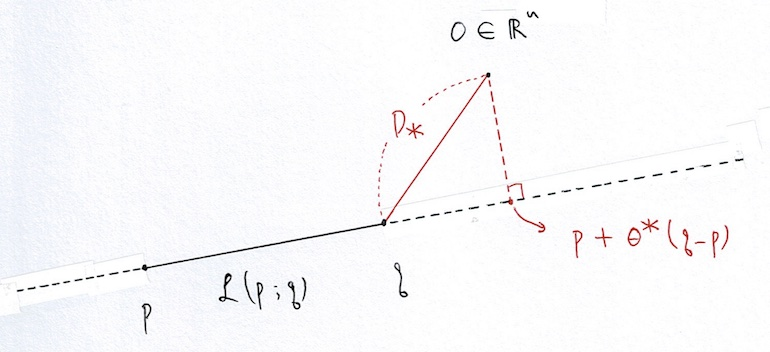
\includegraphics[width=0.5\textwidth]{HW6/figure_problem1_1.jpg}
    \caption{The case for which $\theta^* > 1$ $\Leftrightarrow$ $\mathbf{p}^{\top} \mathbf{q} > \mathbf{q}^{\top} \mathbf{q}$.}
    \label{fig:problem1_1}
    \medskip \ \\
    \medskip
    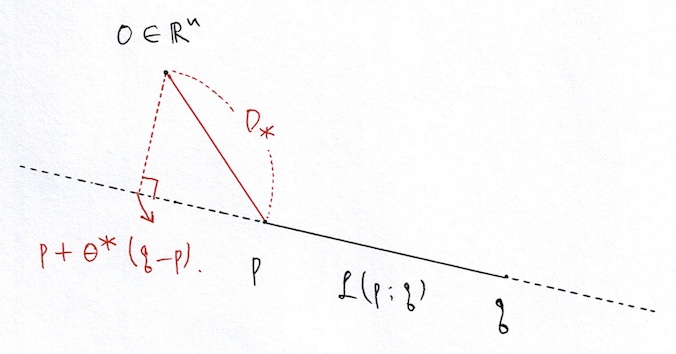
\includegraphics[width=0.5\textwidth]{HW6/figure_problem1_2.jpg}
    \caption{The case for which $\theta^* < 0$ $\Leftrightarrow$ $\mathbf{p}^{\top} \mathbf{q} > \mathbf{p}^{\top} \mathbf{p}$.}
    \label{fig:problem1_2}
    \medskip \ \\
    \medskip
    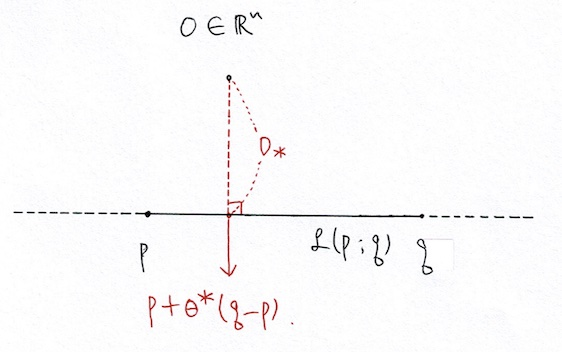
\includegraphics[width=0.5\textwidth]{HW6/figure_problem1_3.jpg}
    \caption{The case for which $0 \leq \theta^* \leq 1$ $\Leftrightarrow$ $\mathbf{p}^{\top} \mathbf{q} \leq \min \left\{ \mathbf{p}^{\top} \mathbf{p}, \mathbf{q}^{\top} \mathbf{q} \right\}$.}
    \label{fig:problem1_3}
\end{figure}
}
\end{problem}

\begin{problem} [\emph{Exercise 9.9} in \cite{calafiore2014optimization}]
\label{problem2}
\normalfont{\ \\
\indent (1) Let $\mathbf{A} := \begin{bmatrix} \mathbf{a}_{1}^{\top} \\ \vdots \\ \mathbf{a}_{n}^{\top} \end{bmatrix} \in \mathbb{R}_{++}^{n \times n}$ and $f(\cdot) : \mathcal{S} := \left\{ \mathbf{x} \in \mathbb{R}^n : \mathbf{x} \succeq \mathbf{0} \textnormal{ and } \mathbf{1}_{n}^{\top} \mathbf{x} = 1 \right\} \rightarrow \mathbb{R}_{++}$, where
\begin{equation*}
    f(\mathbf{x}) := \min \left\{ \frac{\mathbf{a}_{i}^{\top} \mathbf{x}}{x_i} : i \in [n] \right\},
\end{equation*}
where $\mathbf{1}_n \in \mathbb{R}^n$ denotes the $n$-dimensional all-one vector. Here, we adopt the convention that $\frac{\mathbf{a}_{i}^{\top} \mathbf{x}}{x_i} := +\infty$ if $x_i = 0$. Since $\mathcal{S} \subseteq \mathbb{R}_{+}^{n}$ and $f(\mathbf{x}) > 0$ for every $\mathbf{x} \in \mathcal{S}$, it's evident that $f(\mathbf{x}) \cdot \mathbf{x} \succeq \mathbf{0}$, \emph{i.e.}, $f(\mathbf{x}) \cdot \mathbf{x} \in \mathbb{R}_{+}^{n}$. In order to establish $\mathbf{A x} \succeq f(\mathbf{x}) \cdot \mathbf{x}$, it suffices to show that
\begin{equation}
    \label{eqn2.1}
    \left[ \mathbf{Ax} \right]_i - f(\mathbf{x}) \cdot x_i \geq 0,\ \forall i \in [n].
\end{equation}
Indeed, this result holds since
\begin{equation*}
    \begin{split}
        \left[ \mathbf{Ax} \right]_i - f(\mathbf{x}) \cdot x_i = \mathbf{a}_{i}^{\top} \mathbf{x} - f(\mathbf{x}) \cdot x_i
        =
        \begin{cases}
            \mathbf{a}_{i}^{\top} \mathbf{x} & \textnormal{if } x_i = 0; \\
            x_i \left\{ \frac{\mathbf{a}_{i}^{\top} \mathbf{x}}{x_i} - f (\mathbf{x}) \right\} & \textnormal{otherwise.}
        \end{cases}
        \geq 0
    \end{split}
\end{equation*}
for every $i \in [n]$ and $\mathbf{x} \in \mathcal{S}$. This completes the proof of
\begin{equation}
    \label{eqn2.2}
    \mathbf{A x} \succeq f(\mathbf{x}) \cdot \mathbf{x} \succeq \mathbf{0},\ \forall \left( \mathbf{x}, \mathbf{A} \right) \in \mathcal{S} \times \mathbb{R}_{++}^{n \times n}.
\end{equation}
\indent (2) Let $\mathbf{w} \in \mathbb{R}_{++}^{n}$ be a left eigenvector of $\mathbf{A}$ corresponding to a dominant eigenvalue $\lambda = \rho(\mathbf{A}) > 0$, \emph{i.e.}, $\mathbf{w}^{\top} \mathbf{A} = \lambda \mathbf{w}^{\top}$. Since $\mathbf{Ax} - f(\mathbf{x}) \cdot \mathbf{x} \in \mathbb{R}_{+}^n$ for all $\mathbf{x} \in \mathcal{S}$, one has
\begin{equation*}
    \mathbf{w}^{\top} \left\{ \mathbf{Ax} - f(\mathbf{x}) \cdot \mathbf{x} \right\} = \left( \mathbf{w}^{\top} \mathbf{A} \right) \mathbf{x} - f(\mathbf{x}) \left( \mathbf{w}^{\top} \mathbf{x} \right)
    = \left\{ \lambda - f(\mathbf{x}) \right\} \left( \mathbf{w}^{\top} \mathbf{x} \right) \geq 0
\end{equation*}
for every $\mathbf{x} \in \mathcal{S}$. Since $\mathbf{w}^{\top} \mathbf{x} > 0$ for every $\mathbf{x} \in \mathcal{S}$, we obtain $f(\mathbf{x}) \leq \lambda$ for all $\mathbf{x} \in \mathcal{S}$, \emph{i.e.},
\begin{equation}
    \label{eqn2.3}
    \sup \left\{ f(\mathbf{x}) : \mathbf{x} \in \mathcal{S} \right\} \leq \lambda.
\end{equation}
\indent (3) Let $\mathbf{v} \in \mathbb{R}_{++}^{n}$ be a right eigenvector of $\mathbf{A}$ corresponding to a dominant eigenvalue $\lambda = \rho(\mathbf{A}) > 0$, \emph{i.e.}, $\mathbf{Av} = \lambda \mathbf{v}$. Then it's clear that $\mathbf{a}_{i}^{\top} \mathbf{v} = \lambda v_i$ for all $i \in [n]$. Letting $\tilde{\mathbf{v}} := \frac{\mathbf{v}}{\left\| \mathbf{v} \right\|_1}$, it's clear that $\tilde{\mathbf{v}} \in \mathcal{S}$ and
\begin{equation*}
    f \left( \tilde{\mathbf{v}} \right) 
    = \max \left\{ \frac{\mathbf{a}_{i}^{\top} \tilde{\mathbf{v}}}{\tilde{v}_i} : i \in [n] \right\} 
    = \max \left\{ \frac{\mathbf{a}_{i}^{\top} \mathbf{v}}{v_i} : i \in [n] \right\} 
    = \lambda.
\end{equation*}
So we arrive at
\begin{equation*}
    \sup \left\{ f(\mathbf{x}) : \mathbf{x} \in \mathcal{S} \right\} \stackrel{\textnormal{(a)}}{\leq} \lambda = f \left( \tilde{\mathbf{v}} \right)
    \leq \sup \left\{ f(\mathbf{x}) : \mathbf{x} \in \mathcal{S} \right\},
\end{equation*}
where the step (a) follows from the inequality \eqref{eqn2.3}. This yields
\begin{equation*}
    \lambda = \max \left\{ f(\mathbf{x}) : \mathbf{x} \in \mathcal{S} \right\} \quad \textnormal{and} \quad
    \tilde{\mathbf{v}} \in \argmax \left\{ f(\mathbf{x}) : \mathbf{x} \in \mathcal{S} \right\},
\end{equation*}
as desired.
}
\end{problem}

\newpage

\bibliographystyle{plain}
\bibliography{main.bib}

\end{document}